\documentclass[xcolor={dvipsnames}]{beamer}%[handout] slides non ripetute

\usetheme{Singapore}
\usecolortheme{rose}

\usepackage[utf8]{inputenc}	%lettere accentate
\usepackage[italian]{babel}	%sillabazione italiana
\usepackage{amsmath}		%simboli matematici
\usepackage{amsfonts}		%font matematici
\usepackage{amssymb}		%altri simboli matematici
\usepackage{tikz}			%grafica
\usepackage{subfloat}		%affiancare figura
\usepackage{cancel}			%simbolo di semplificazione
\usepackage{pdfpages}		%incorporare pdf
\usepackage{soul}			%testo barrato
\usepackage{listings}		%codice


\definecolor{back}{rgb}{0.93,0.93,0.97} 

\lstset{ %
	backgroundcolor=\color{back},  	% choose the background color; you must add \usepackage{color} or \usepackage{xcolor}; should come as last argument
	basicstyle=\tiny,        		% the size of the fonts that are used for the code
	breakatwhitespace=false,        % sets if automatic breaks should only happen at whitespace
	breaklines=true,                % sets automatic line breaking
	captionpos=b,                   % sets the caption-position to bottom
	commentstyle=\color{gray},   	% comment style
	frame=single,	                % adds a frame around the code
	keepspaces=true,                % keeps spaces in text, useful for keeping indentation of code (possibly needs columns=flexible)
	keywordstyle=\color{blue},      % keyword style
	language=Python,               	% the language of the code
	numbers=none,                   % where to put the line-numbers; possible values are (none, left, right)
	numbersep=5pt,                  % how far the line-numbers are from the code
	numberstyle=\tiny\color{black}, % the style that is used for the line-numbers
	rulecolor=\color{black},        % if not set, the frame-color may be changed on line-breaks within not-black text (e.g. comments (green here))
	showspaces=false,               % show spaces everywhere adding particular underscores; it overrides 'showstringspaces'
	showstringspaces=false,         % underline spaces within strings only
	showtabs=false,                 % show tabs within strings adding particular underscores
	stepnumber=1,                   % the step between two line-numbers. If it's 1, each line will be numbered
	stringstyle=\color{OrangeRed},  % string literal style
	tabsize=2                   	% sets default tabsize to 2 spaces
}

\newcommand{\codice}[2]{\lstinputlisting[firstline=#1, lastline=#2]{code/PCA.py}}
\newcommand{\figcen}[2]{
	\begin{figure}
		\begin{center}
			\includegraphics[width=#1]{#2}
		\end{center}
	\end{figure}
}

\author{Marco Buracchi}

\title{Principal Component Analysis:\\ dalla teoria alla pratica}

\institute{Università degli studi di Firenze}

\date{\today}

\subject{Multivariate Analysis and Statistical Learning}

%\setbeamercovered{transparent}

\setbeamertemplate{navigation symbols}{}
\setbeamertemplate{caption}[numbered]
\setbeamerfont{caption}{size=\scriptsize}

\graphicspath{{img/}}

\logo{\includegraphics[scale=0.03]{logo.eps}}

\begin{document}

\maketitle

\small

\begin{frame}{Sommario}

  \tableofcontents

\end{frame}

\section{Principal Component Analysis}

	\begin{frame}{PCA}
		\begin{itemize}
			\item Trasformazione lineare della matrice dei dati $\mathcal{X}$
			\item Misurazione della variazione delle variabili utilizzando un numero minore di "fattori"
			\item Trasportare il problema in uno spazio \emph{k}-variato (generalmente bi-trivariato)
			\item Semplificazione di visualizzazione e lettura dei dati
		\end{itemize}
	\end{frame}

	\subsection{Cosa fa?}
		\begin{frame}{Esempio}
			\begin{columns}
				\begin{column}{0.5\textwidth}
					\figcen{\columnwidth}{plotTeoria}
				\end{column}
				\begin{column}{0.5\textwidth}
					\begin{itemize}
						\item 40 campioni
						\item 2 variabili
					\end{itemize}
				\end{column}
			\end{columns}			
		\end{frame}
	
		\begin{frame}{Esempio - 2}
			\figcen{.8\textwidth}{proiezione}
			\begin{itemize}
				\item Nessuna delle due variabili descrive completamente la variabilità dei dati
			\end{itemize}
		\end{frame}
	
		\begin{frame}{Componenti}
			\figcen{.7\textwidth}{componenti}
			\begin{itemize}
				\item Prendiamo come componenti principali le linee blu
				\item La prima componente spiega la massima percentuale di variabilità rappresentabile in una dimensione
			\end{itemize}
		\end{frame}
	
		\begin{frame}{Varianza}
			\begin{itemize}
				\item Questa percentuale di variabilità può essere calcolata tramite la varianza
				\item La varianza è un indice della dispersione dei dati lungo una particolare direzione
				\item La varianza è indipendente dal sistema di riferimento
				\item Ruotare gli assi mantiene inalterata la varianza totale
			\end{itemize}
		\end{frame}
	
		\begin{frame}{Componenti - 2}
			\begin{itemize}
				\item La prima componente cattura quasi tutta la variabilità presente nei dati (99.83\%)
				\item La seconda descrive la rimanente (0.17\%)
				\item Generalizzando, le componenti principali successive spiegano una sempre minore percentuale della variabilità originale
				\item Le ultime componenti principali descrivono principalmente rumore
			\end{itemize}
		\end{frame}
		
	\subsection{Come funziona?}
		\begin{frame}{Funzionamento}
			\begin{enumerate}
				\item Standardizzazione
				\begin{itemize}
					\footnotesize
					\item Standardizzare i dati (media = 0, varianza = 1)
					\item Possiamo lavorare con variabili su scale e unità di misure differenti
				\end{itemize}
				\item Calcolo covarianza/correlazione
				\begin{itemize}
					\footnotesize
					\item Calcoliamo la matrice S di covarianza $$\mathcal{S} = \frac{1}{n-1} \sum_{1}^{n} (x-\mu)(x-\mu)^T$$
					\item Possiamo usare anche la matrice di correlazione
				\end{itemize}
				\item Calcolo autovalori/autovettori 
				\begin{itemize}
					\item $\mathcal{S} \times v = \lambda \times v$
				\end{itemize}
			\end{enumerate}
		\end{frame}
	
		\begin{frame}{Funzionamento}
			\begin{enumerate}
				\setcounter{enumi}{3}
				\item Scelta delle componenti
				\begin{itemize}
					\footnotesize
					\item Ordiniamo in maniera decrescente gli autovalori ottenuti
					\item Selezioniamo i primi \emph{k}
					\item Costruiamo $\mathcal{V}$, la matrice dei rispettivi autovettori
				\end{itemize}
				\item Rotazione dei dati
				\begin{itemize}
					\footnotesize
					\item Moltiplichiamo i dati originali per gli autovettori che indicano le direzioni dei nuovi assi (componenti principali) 
					\item I dati ruotati vengono chiamati \emph{score} $$Sc = \mathcal{X} \times \mathcal{V}$$
				\end{itemize}
			\end{enumerate}
		\end{frame}
	
\section{Implementazione Python}

	\subsection{Strumenti}

	\begin{frame}{Strumenti utilizzati}
		\begin{itemize}
			\item Linguaggio: Python
			\item Libreria per l'analisi dei dati: \emph{PANDAS}
			\item Dataset: IRIS
		\end{itemize}
	\end{frame}

	
	\begin{frame}{PANDAS}
		\begin{itemize}
			\item Libreria Python, open source, ad alte prestazioni e con licenza BSD
			\item Strutture dati e strumenti per l'analisi facili da usare (R-like)
			\begin{itemize}
				\footnotesize
				\item Serie (unidimensionali)
				\item Dataframe (bidimensionali)
			\end{itemize}
			\item Dati organizzati in maniera \emph{relazionale} o \emph{etichettata}
			\item Sponsorizzato da NumFocus
			\begin{columns}
				\begin{column}{.3\textwidth}
					\figcen{\columnwidth}{numFocus}
				\end{column}
				\begin{column}{.7\textwidth}
					\begin{itemize}						
						\footnotesize
						\item sviluppo continuo, a livello mondiale e sistema di donazioni a supporto
					\end{itemize}						
				\end{column}
			\end{columns}
		\end{itemize}
	\end{frame}
	
	\begin{frame}{Dataset}
		\begin{columns}
			\begin{column}{.6\textwidth}
				\figcen{\columnwidth}{iris}
			\end{column}
			\begin{column}{.5\textwidth}
				\begin{itemize}
					\item Dataset IRIS
					\item 150 misurazioni di fiori iris 
					\item 3 diverse specie
				\end{itemize}
			\end{column}
		\end{columns}
	\end{frame}

	\subsection{Implementazione}
	
		\begin{frame}{Caricamento Dataset}
			\codice{16}{25}
			\figcen{.7\textwidth}{tab}
		\end{frame}
	
		\begin{frame}{Divisione valori}
			\begin{itemize}
				\item Matrice valori numerici $X \in \mathcal{M}^{150x4}$
				\item Vettore specie $y \in \mathcal{M}^{150x1}$
			\end{itemize}
			\codice{30}{32}
		\end{frame}
	
		\begin{frame}{Analisi descrittiva}
			\codice{37}{56}
		\end{frame}
	
		\begin{frame}{Analisi descrittiva}
			\figcen{.8\textwidth}{isto}
		\end{frame}
	
		\begin{frame}{Analisi descrittiva}
			\begin{itemize}
				\item Valori su scale diverse richiedono standardizzazione
				\item Usiamo la funzione di libreria
			\end{itemize}
			\codice{58}{59}
		\end{frame}
	
		\begin{frame}{Autovalori e autovettori}
			\codice{61}{82}
		\end{frame}
	
		\begin{frame}{Autovalori e autovettori}
			\codice{84}{94}
			\begin{itemize}
				\item In tutti i casi otteniamo la matrice $$\begin{bmatrix}
				0.52237162 & -0.37231836 & -0.72101681 & 0.26199559\\
				-0.26335492 & -0.92555649 & 0.24203288 & -0.12413481\\
				0.58125401 & -0.02109478 & 0.14089226 & -0.80115427\\
				0.56561105 & -0.06541577 & 0.6338014 & 0.52354627\\
				\end{bmatrix}$$
			\end{itemize}
		\end{frame}
	
		\begin{frame}{Selezione componenti}
			\begin{itemize}
				\item Gli autovettori calcolati forniscono solamente la direzione perché sono tutti a norma unitaria
				\item Per scegliere i più interessanti ordiniamo i rispettivi autovalori
			\end{itemize}
			\codice{96}{102}
		\end{frame}
	
		\begin{frame}{Varianza spiegata}
			\begin{itemize}
				\item Calcoliamo la varianza spiegata dalle singole componenti
				\item Visualizziamo il risultato su un grafico
			\end{itemize}
			\codice{108}{123}
		\end{frame}
	
		\begin{frame}{Varianza spiegata}
			\figcen{.9\textwidth}{istoVarianza}
		\end{frame}
	
		\begin{frame}{Matrice di proiezione}
			\begin{itemize}
				\item Passiamo da 4 a 2 dimensioni
				\item Estraiamo le prime due componenti dalla matrice degli autovettori
			\end{itemize}
			\codice{125}{127}
			\begin{itemize}
				\item Creiamo la matrice di proiezione $\mathcal{W}$
			\end{itemize}
			$$\mathcal{W} = \begin{bmatrix}
			0.52237162 & -0.37231836\\
			-0.26335492 & -0.92555649\\
			0.58125401 & -0.02109478\\
			0.56561105 & -0.06541577\\
			\end{bmatrix}$$
		\end{frame}
	
		\begin{frame}{Proiezione}
			\begin{itemize}
				\item Proiettiamo nel nuovo sottospazio $$\mathcal{Y} = \mathcal{X}\times \mathcal{W} \qquad \mathcal{Y} \in \mathcal{M}^{150x2}$$
			\end{itemize}
			\codice{132}{133}
		\end{frame}
	
		\begin{frame}{Risultato}
			\figcen{.8\textwidth}{PCA}
		\end{frame}
	
		\begin{frame}{Post Scriptum}
			\begin{itemize}
				\item Esiste una funzione di libreria che calcola $\mathcal{Y}$ direttamente da $\mathcal{X}$
				\item L'unico parametro da fornire è il numero di componenti che si vogliono prendere in considerazione
			\end{itemize}
			\codice{149}{151}
			\figcen{.3\textwidth}{ok}
		\end{frame}

\section{Caso di studio}
	\begin{frame}{Caso di studio}
		Caso di studio
	\end{frame}

	\subsection{Attacchi}
		\begin{frame}{Attacco SMURF}
			\begin{figure}
				\begin{center}
					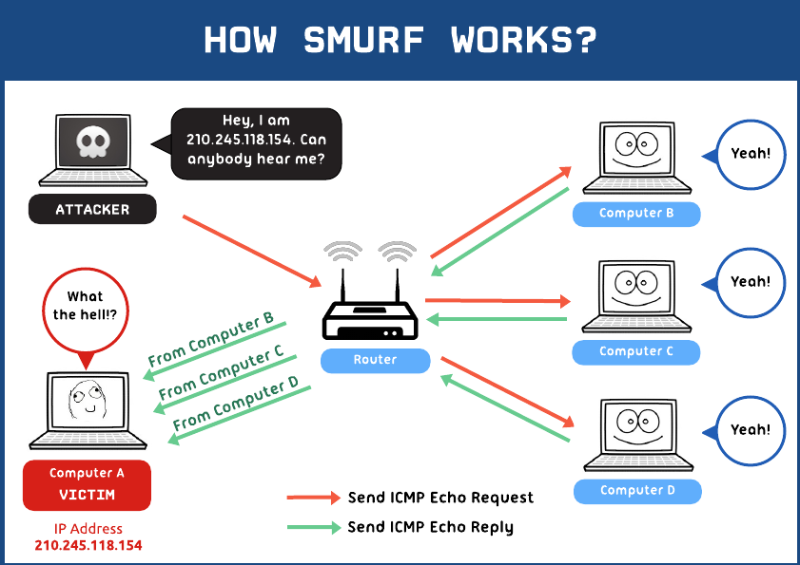
\includegraphics[width=.75\textwidth]{smurf}
				\end{center}
			\end{figure}
		\end{frame}
		\begin{frame}{Attacco Neptune}
			\begin{figure}
				\begin{center}
					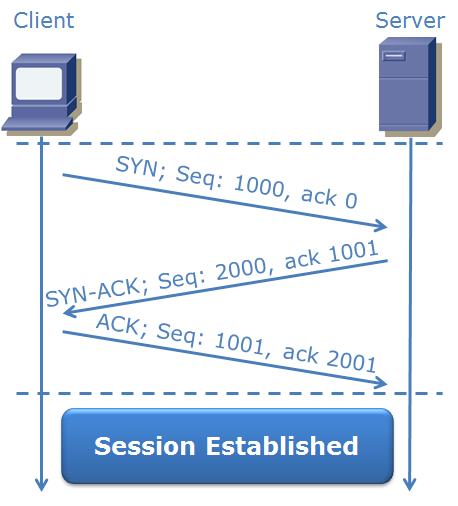
\includegraphics[width=.5\textwidth]{3wayh}
				\end{center}
			\end{figure}
		\end{frame}
		
		\begin{frame}{Attacchi Network Probe}
			NP
		\end{frame}
	
	\subsection{Analisi}
		\begin{frame}{Analisi}
			Preprocessing
		\end{frame}
	
	\subsection{Risultati}
		\begin{frame}{Rilevazione}
			Rilevazione
		\end{frame}

	\begin{frame}{Bibliografia}
	{
		\scriptsize
		\nocite{anderson2003introduction,mardia1979multivariate,pandasManual,pandasSite,Labib2006}
		\bibliography{bibliografia}
		\bibliographystyle{unsrt}
	}
	\end{frame}

\end{document}
